\documentclass[12pt]{report}
\usepackage[utf8]{inputenc}
\usepackage{outline}
\usepackage{amsfonts}
\usepackage{pmgraph}
\usepackage{afterpage}
\usepackage{amsfonts}
\usepackage{amsmath,amssymb,amsthm}
\usepackage{bigstrut}
\usepackage{caption}
\usepackage[english]{babel}
\usepackage{cite}
\usepackage{float}
\usepackage{geometry}
\usepackage{graphicx}
\usepackage{hyperref}
\usepackage[utf8]{inputenc}
\usepackage{listings}
\usepackage{mathtools}
\usepackage{subcaption}
\usepackage{tabularx}
\usepackage{titlesec}
\usepackage{wrapfig}
\usepackage{bm}
\usepackage{listings}
\usepackage[normalem]{ulem}
\title{\textbf{Redes Neurais II Segunda Lista de Exercícios}}
\author{Lucas Oliveira David\\ld492@drexel.edu\\188972}
\date{\oldstylenums{24}/\oldstylenums{11}/\oldstylenums{2016}}

\setlength{\oddsidemargin}{0in}
\setlength{\evensidemargin}{0in}
\setlength{\topmargin}{0in}
\setlength{\headsep}{-.25in}
\setlength{\textwidth}{6.5in}
\setlength{\textheight}{8.5in}

\setlength{\parindent}{1cm}

\usepackage{color}

\definecolor{codegreen}{rgb}{0,0.6,0}
\definecolor{codegray}{rgb}{0.5,0.5,0.5}
\definecolor{codepurple}{rgb}{0.58,0,0.82}
\definecolor{backcolour}{rgb}{0.95,0.95,0.92}

\lstdefinestyle{mystyle}{
	backgroundcolor=\color{backcolour},   
	commentstyle=\color{codegreen},
	keywordstyle=\color{magenta},
	numberstyle=\tiny\color{codegray},
	stringstyle=\color{codepurple},
	basicstyle=\footnotesize,
	breakatwhitespace=false,         
	breaklines=true,                 
	captionpos=b,                    
	keepspaces=true,                 
	numbers=left,                    
	numbersep=5pt,                  
	showspaces=false,                
	showstringspaces=false,
	showtabs=false,                  
	tabsize=2
}

\lstset{style=mystyle}

\begin{document}

\maketitle

\section{1. Classificador probabilístico}

\subsection{(a) Arquitetura}

A arquitetura do classificador pode ser descrita pela equação \ref{eq:clf-prob}, que seleciona a classe $i$ de menor custo $F_i$ associado.

\begin{align}
	\label{eq:clf-prob}
	\begin{split}
		y(x) &= \arg_i \min \{F_i(x) \mid 1 \le i \le N\}\\
		F_i(x) &= R(\alpha_i \mid x)\\
		&= \sum_{j \ne i} P(C_i \mid x)
	\end{split}
\end{align}

\subsection{(b) Critério MAP}

\begin{figure}[H]
	\centering
	\includegraphics[width=.5\textwidth]{assets/map}
	\caption{Densidades ponderadas, seguindo o critério MAP.}
	\label{fig:map}
\end{figure}

Onde a função de decisão pode ser definida por:

\[
y(x)= 
\begin{cases}
-1, & \text{se } 0 \le x \le 1 \\
+1, & \text{caso contrário}
\end{cases}
\]

Finalmente, para a probabilidade de escolha correta:

\begin{align*}
	P_{\text{correta}} &= \sum_{i = 1}^2 \int_{R_i} p(x \mid C_i) dx \times p(C_i) \\
	&= 0.354024803716 + .6\\
	&= 0.954024804
\end{align*}

\subsection{(c) Critério MV}

\begin{figure}[H]
	\centering
	\includegraphics[width=.5\textwidth]{assets/mv}
	\caption{Densidades ponderadas, seguindo o critério MV.}
	\label{fig:mv}
\end{figure}

Aqui, a relação de entre as duas funções de densidade probabilística se mantém em relação ao seu comportamento pelo critério MAP. A função de decisão é portanto a mesma. Já a probabilidade de escolha correta é:

\begin{align*}
	P_\text{correta} &= 0.442531004645 + 0.545454545455 \\
	&= 0.987985550100
\end{align*}

\subsection{(d) Comparação entre os dois critérios (MAP e MV)}

As probabilidades de acerto encontradas para ambos os critérios são consideravelmente próximas, com o MV na frente por uma margem de aproximadamente 3\%. Entretanto, também se nota --- por inspeção visual --- que ambos os critérios produziram as mesmas regiões de decisão para o modelo. Portanto, essa diferença de probabilidades de acerto é provavelmente causada pelo processo de integração numérica, feito pelo método de Simpson e considerando 100 observações no intervalo $[-3, 6]$.

\section{2. Problema extraído do \textit{UCI Repository}}

\subsection{(a) Escolha do conjunto de dados}

O conjunto de dados escolhido, denominado \textbf{Adult Data Set}, contém 48842 amostras que descrevem individuos por 15 características, como descritas abaixo:
		
\begin{itemize}
	\item age: a idade do invidíduo.
	\item type-employer: o tipo empregatício do indivíduo (e.g. government, military, private).
	\item fnlwgt: número de pessoas que os participantes acreditam a observação representar.
	\item education: o maior nível de educação alcançado pelo indivíduo.
	\item education-num: o maior nível de educação em forma numérica.
	\item marital: status matrimonial do indivíduo (e.g. Never-married, Separated).
	\item occupation: a ocupação do invidíduo.
	\item relationship: status de relacionamento (e.g. Husband, Unmarried, Wife).
	\item race: grupo étnico do invidíduo (e.g. Black, White, Eskimo).
	\item sex: grupo biológico do indivíduo (e.g. Female, Male).
	\item capital-gain: ganhos capitais observados.
	\item capital-loss: perda captais observados.
	\item hr-per-week: horas semanais trabalhadas.
	\item country: país de origem do indivíduo.
	\item income: variável Booleana indicando se o indivíduo faz mais
	de \$50,000 anualmente (e.g. $\le 50K$, $>50K$).
\end{itemize}
		
Dois fatores importantes levados em consideração na escolha de \textbf{Adult} foram a ocorrência de valores categoricos como atributos alimentados à máquina de inferência e a pontual falta de alguns valores em alguns indivíduos. As técnicas descritas a seguir foram empregadas no pre-processamento dos dados, a fim de lidar com tais peculiaridades:
		
\begin{itemize}
	\item \textbf{Imputing:} algumas instâncias possuem valores indefinidos --- indicados por \textit{'?'} --- para algumas de suas características. Novamente, estes elementos . Várias estratégias podem ser adotadas para contornar este problema. Por exemplo: simplesmente desconsiderar todas as amostras que apresentarem ao menos um valor indefinido ou criar um novo valor de característica e associá-lo a cada um dos indivíduos com valor faltante.
	
	Neste trabalho, a estratégia "mediana" foi adotada, onde o valor válido mais próximo à média é utilizado para substituir as indeterminações. Esta estrategia é interessante visto que gera valores válidos e médios (que serão portanto pouco importantes no processo de inferência, amenizando as possíveis interferências criadas a partir desta suposição). Como exemplo, a característica \textit{workclass}:
	\begin{lstlisting}[label={lst:label}, caption={Possíveis valores para as características \textit{workclass}. Note que ao menos uma amostra do conjunto possue o valor indefinido para esta classe, já que \textit{?} foi identificado como um dos valores possíveis. Em seguida, observa-se exemplos de como tais classes foram mapeadas para números.}]
	workclass: ?, Federal-gov, Local-gov, Never-worked, Private,
	Self-emp-inc, Self-emp-not-inc, State-gov, Without-pay
	examples: [ 7.  6.  4. ...,  4.  4.  5.]
	\end{lstlisting}
	
	\item \textbf{Label encoding}, isto é, a conversão de características nominais para números é fundamental na fase de pre-processamento, tendo em vista que as máquinas aqui utilizadas são essencialmente numéricas. Isto pode ser feito, para cada característica, a partir de uma enumeração qualquer do conjunto composto por possíveis valores desta mesma. Por exemplo, a Listagem \ref{lst:featuresenum} exibe uma possível enumeração do atributo \textit{income}, onde $0$ é associado à classe "$\le50K$" e o $1$ à classe "$>50K$".
	
	\begin{lstlisting}[label={lst:featuresenum}, caption={Possível enumeração para a característica \textit{income}.}]
	income: <=50K, >50K
	examples: [ 0.  0.  0. ...,  0.  0.  1.]
	\end{lstlisting}
	
	\item \textbf{One Hot Encoding:} ao mapearmos os atributos categóricos das amostras para números, podemos imediatamente utilizá-las para treinar um modelo de aprendizado utilizando métodos numéricos. Se o fizéssemos, entretanto, transportaríamos para o nosso modelo uma forte suposição: a ordenação do conjunto dos naturais. Considere, como exemplo, um atributo \textit{color} que assume os valores \textit{red}, \textit{blue} e \textit{green}. Sejam amostras $x, y$ e $z$ tais que cada uma possui um dos valores possíveis. Ao codificar estes valores, estaríamos necessariamente dizendo que $x$ está espacialmente mais próximo à $y$ do que à $z$, o que não é necessariamente verdade.
	
	A fim de lidar com esta suposição, cada valor $0 \le i < n$ pode ser traduzido como uma sequência de bits de tamanho $n$, onde somente o bit $i$ assume valor $1$. Exemplo:
	
	\begin{lstlisting}[label={lst:label}]
x := (0)
y := (1)
z := (2)
x', y', z' = one-hot-encode((x, y, z))
x' = (0, 0, 1), y' = (0, 1, 0), z' = (1, 0, 0)
	\end{lstlisting}
	
	Todas as características estão a`ora à mesma distância umas das outras. Se considerarmos a $L_2$, por exemplo:
	
	$$\|x' - y'\| = \|(0, 0, 1) - (0, 1, 0)\| = \sqrt{2} = \|(0, 0, 1) - (1, 0, 0)\| = \|x' - z'\|$$
	
	Nota-se que, na prática, este procedimento altera o número de características do conjunto de dados. Ele portanto não é aplicado na atividade (c), onde estamos interessados na seleção dentre os atributos originais.
\end{itemize}
		
Finalmente, dentre diversas tarefas possíveis sobre o conjunto \textbf{Adult}, nos focaremos na predição da característica \textit{income} a partir das demais. Isto é, um problema de discriminação binária. Figura \ref{fig:adult_ds} ilustra o conjunto Adult discriminado pelo atributo \textit{income}.
				
\begin{figure}[H]
	\centering
	\begin{subfigure}[b]{0.45\textwidth}
		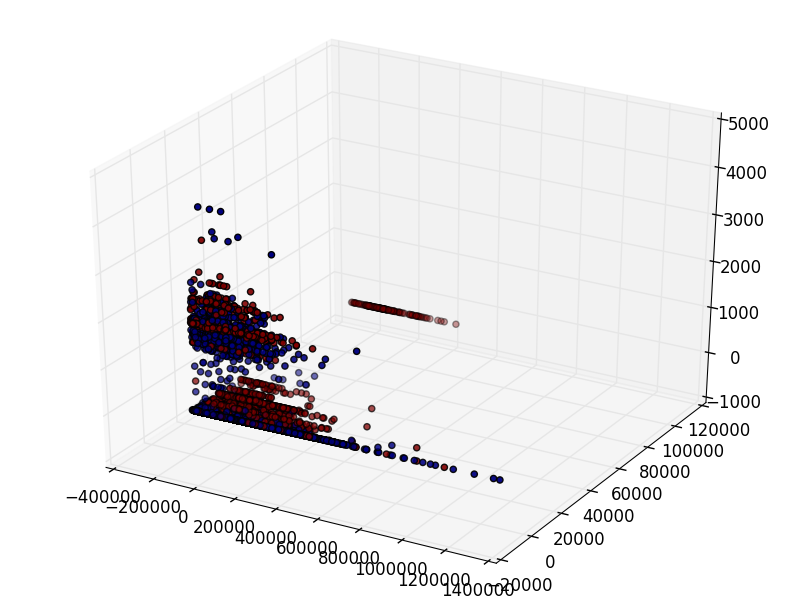
\includegraphics[width=\textwidth]{assets/train-data}
		\caption{Conjunto de treinamento.}
		\label{fig:ds_adult_train}
	\end{subfigure}
	~\begin{subfigure}[b]{0.45\textwidth}
		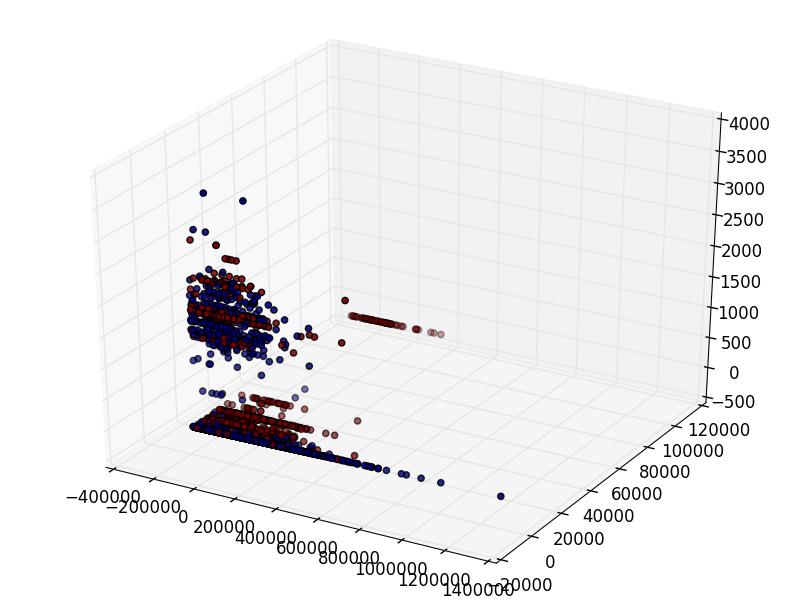
\includegraphics[width=\textwidth]{assets/test-data}
		\caption{Conjunto de teste.}
		\label{fig:ds_adult_test}
	\end{subfigure}
	\caption{Conjuntos de treinamento e teste de \textbf{Adult}, preprocessados com \textit{PCA}, onde a cor de cada amostra representa o atributo \textit{income}.}\label{fig:adult_ds}
\end{figure}

\subsection{(b) Separação de dados treino/validação/teste}
O conjunto possui uma distinção física (dois arquivos distindos), fazendo a separação entre \textbf{treino} e \textbf{teste}. Foi suposto, por hipótese, que essa separação é ótima e aleatória. No que diz respeito ao treinamento utilizando \textit{Extreme Learning Machines}, o conjunto \textbf{treino} foi aleatoriamente sub-dividido em dois subconjuntos \textbf{treino'} e \textbf{val}, onde \textbf{treino'} contina 70\% das amostras do conjunto original, enquanto \textbf{val} continha o restante.
Já para o treinamento do modelo utilizando o discriminante de Fisher, nenhuma divisão do conjunto de treinamento foi feita -- visto que não há hiperparâmetros a serem otimizados.
Finalmente, para o treinamento da SVM, o conjunto de treinamento foi dividido em três subconjuntos disjuntos e esses foram utilizados para treinar e validar os modelos pela estratégia \textit{3-fold cross validation}.
		
% Note que se o balanceamento de classes é descrito pela probabilidade $p$ de uma amostra $x \in \bm X$ pertencer à classe $1$, então um \textit{sampling} aleatório de $\bm X$ pouco afeta o balanceamento de classes original. Isto é, seja $X'$ um subconjunto de $X$ e $x' \in X'$, $P[y(x') = 1] \approx p$.

\subsection{(c) Seleção de atributos por filtragem}
		
Ao calcular a covariância Pearson $R(j)$ para cada atributo $j$ (Tabela \ref{tbl:features-pearson}), nota-se que a covariância absoluta acumulada é maior que 96\% já para os 10 primeiros atributos. Isto é,
		
$$\frac{\sum_{i=1}^{10} |R(j)|}{\sum_{i=1}^{14} |R(j)|} \ge 0.96$$
		
\begin{table}[H]
	\centering
	\begin{tabular}{lr}
		educationnum  & 0.34  \\
		relationship  & -0.25 \\
		age           & 0.23  \\
		hoursperweek  & 0.23   \\
		capitalgain   & 0.22  \\
		sex           & 0.22  \\
		maritalstatus & -0.19 \\
		capitalloss   & 0.15  \\
		education     & 0.08  \\
		race          & 0.07  \\
		occupation    & 0.05  \\
		nativecountry & 0.02  \\
		fnlwgt        & -0.01 \\
		workclass     & 0.00
	\end{tabular}
	\caption{Covariância Perason entre cada um dos atributos considerados e o atributo \textit{income}, ordenados decrescentemente por valor absoluto.}
	\label{tbl:features-pearson}
\end{table}
		
Com base nessa informação, selecionamos os 10 primeiros atributos (considerando a ordenação imposta na Tabela \ref{tbl:features-pearson}) de todos os possíveis.

\subsection{(d) Aprendizado com \textit{Extreme Learning Machines}}

O seguinte pipeline de pré-processamento dos dados foi adotado:

\begin{enumerate}
	\item \textbf{Missing imputing:} valores faltantes eram substituídos pelo valor mediano do atributo, com respeito à todas as amostras. Se nenhuma amostra contivesse um valor válido para um determinado atributo, este atributo seria completamente removido (este não foi o caso para o conjunto \textbf{Adult}).
	\item \textbf{One-hot-encoding:} conversão de valores naturais para vetores unitários, resultando em uma transformação do conjunto com 14 características para um outro com 105.
	\item \textbf{Principal Component Analysis:} encontrar as 10 principais componentes principais do conjunto, que ``explicam" 99.99\% da variância dos dados.
\end{enumerate}

É importante destacar que as transformações feitas sobre o conjunto de teste foram ajustadas a partir dos parâmetros do conjunto de treinamento. Por exemplo, as componentes principais utilizadas para transformar o conjunto de testes foram encontradas a partir (e somente) do conjunto de treinamento. A razão para isto é não agregar informação do conjunto de testes aos nossos modelos, possivelmente comprometendo o método de avaliação.

\begin{table}[H]
	\centering
	\begin{tabular}{|l|r|r|}
		\hline
		\textbf{Parâmetros} & \textbf{Acurácia em treino} & \textbf{Acurácia em teste} \\\hline
		1024 unidades cam. interna; $\lambda = 0.01$ & 84\% & 84\% \\\hline
		4096 unidades cam. interna; $\lambda = 0.01$ & 84\% & 84\% \\\hline
		8192 unidades cam. interna; $\lambda = 0.01$ & 84\% & 84\% \\\hline
		1024 unidades cam. interna; $\lambda = 0.1$  & 80\% & 80\% \\\hline
		1024 unidades cam. interna; $\lambda = 0.5$  & 76\% & 77\% \\\hline		
		1024 unidades cam. interna; $\lambda = 0.9$  & 76\% & 76\% \\\hline
	\end{tabular}
	\caption{Pontuações dos diferentes parâmetros buscados para a \textit{Extreme Learning Machine}.}
	\label{tbl:lrn_em_scores}
\end{table}

Ao observar as perdas de cada modelo na Figura \ref{fig:em_train_losses}, nota-se que o aumento no número de unidades na camada interna afeta unicamente o tempo de treinamento.

\begin{figure}[H]
	\centering
	\begin{subfigure}[b]{.95\textwidth}
		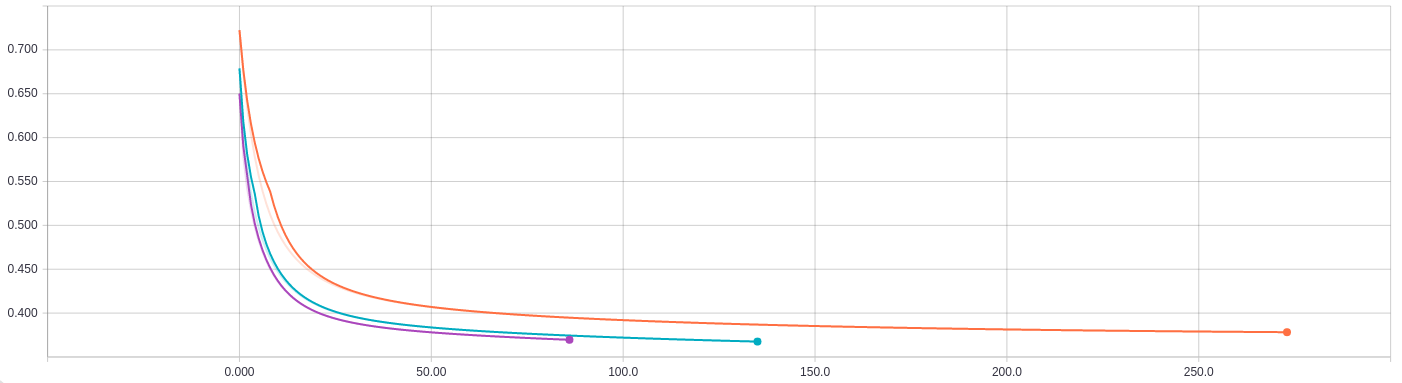
\includegraphics[width=\textwidth]{assets/train}
		\caption{\textit{Cross-entropy loss} sobre o conjunto de treinamento/\textit{epoch}.}
		\label{fig:em_loss}
	\end{subfigure}
	~\begin{subfigure}[b]{.95\textwidth}
		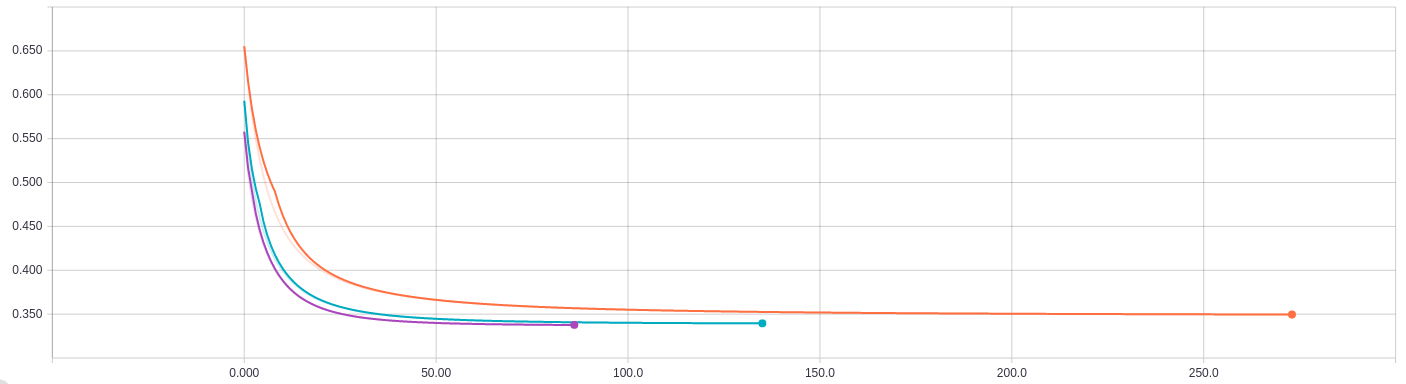
\includegraphics[width=\textwidth]{assets/val}
		\caption{\textit{Cross-entropy loss} sobre o conjunto de validação/\textit{epoch}.}
		\label{fig:em_val_loss}
	\end{subfigure}
	\caption{\textit{Cross-entropy loss} sobre ambos conjuntos (treinamento e validação). As três curvas representam os seguintes modelos: roxo -- 1024 unidades na cam. interna; azul -- 4096 unidades na cam. internas; laranja -- 8192 unidades na cam. interna.}
	\label{fig:em_train_losses}
\end{figure}

\subsection{(e) Aprendizado com \textit{Fisher's Discriminant}}

Reutilizamos aqui o mesmo pré-processamento empregado no item (d) Aprendizado com \textit{Extreme Learning Machines}. Ademais, nenhuma otimização de hiperparâmetros foi necessária, tendo em vista a natureza do algoritmo de aprendizagem do modelo (Listagem \ref{lst:fisher}).

\begin{lstlisting}[language=Python, caption={Construção do modelo baseado no discriminante de Fisher. Ao final, as variáveis $W$ e $b$ conterão os parâmetros do modelo.}, label={lst:fisher}]
X_0, X_1 = X[y == 0], X[y == 1]
u0, u1 = np.mean(X_0, axis=0), np.mean(X_1, axis=0)

Sw = (X_0 - u0).T.dot(X_0 - u0) + (X_1 - u1).T.dot(X_1 - u1)
W = np.linalg.inv(Sw).dot(u1 - u0)
b = (W.T.dot(u0) + W.T.dot(u1)) / 2
\end{lstlisting}

O modelo gerado a partir dos parâmetros $W$ e $b$ encontrados obteve uma acurácia de 79\% sobre ambos conjuntos de treinamento e teste.

\subsection{(f) Aprendizado com uma \textit{SVM}}

Mas uma vez, reutilizamos o pré-processamento descrito em (d). Entretanto, a busca pelos melhores parâmetros se deu através da técnica de \textit{grid search}, onde a pontuação de validação é calculada para cada combinação de parâmetros possível e a melhor configuração é selecionada.

O espaço de busca utilizado neste experimento é descrito pelo conjunto abaixo:

$$S = \{(C, kernel) \mid C \in (.01, .1, 1, 10, 100), kernel \in (linear, rbf)\}$$

Da busca descrita acima, obtivemos que os parâmetros K = 'rbf' e $C = 100$ como maiores pontuadores sobre o conjunto de validação, produzindo as seguintes acurácias:

\begin{table}[H]
	\centering
	\begin{tabular}{l|r|r|r}
		\textbf{Parâmetros} & \textbf{Acc treino} & \textbf{Acc. validação} & \textbf{Acc teste} \\\hline
		kernel = 'rbf'; $C = 100$ & 83\% & 80\% & 80\%  \\
	\end{tabular}
	\caption{Pontuações do melhor conjunto de parâmetros para o \textit{SVM}.}
	\label{tbl:lrn_svm_scores}
\end{table}

\subsubsection{(g) Comparação entre os classificadores}

Dentre todos os modelos de aprendizagem testados, nota-se uma mais alta taxa de acurácia para as \textit{Extreme Learning Machines}, que alcançaram 84\% sobre o conjunto de teste. Os \textit{SVMs} ficam em segundo lugar, alcançando 80\% de acurácia. Em último lugar se encontra o modelo baseado no discriminante de Fisher, com apenas 74\% de acurácia sobre o conjunto teste.

\end{document}
